\label{chap:teoria}

In questo capitolo ci focalizzeremo sulla parte del Machine Learning che si
occupa del processo di creazione di modelli in grado di apprendere
autonomamente dai dati. Un modello è costituito da un insieme di parametri e
una struttura di calcolo che tratta i dati di input per produrre un output. I
parametri vengono appresi durante la fase di addestramento, in cui il modello
esamina vari esempi e regola i propri parametri in modo da rendere minima una
funzione costo. Gli iperparametri, d'altra parte, sono valori definiti
dall'utente prima dell'inizio dell'addestramento che influenzano la struttura
del modello e il suo comportamento durante l'addestramento.

Prima di esplorare i modelli specifici, ci concentreremo sul processo di
creazione dei modelli di Machine Learning, e vedremo come l'automatizzazione
di questo processo, attraverso l'impiego di una pipeline, possa migliorarne
l'efficienza e l'efficacia.

Il processo di creazione di un modello di Machine Learning si compone di vari
passaggi: l'estrazione dei dati, la loro preparazione e l'addestramento del
modello. Una pipeline collega questi passaggi in sequenza, incapsulandoli in
un'entità che, dall'esterno, può essere utilizzata come se fosse il modello
stesso. Questa pipeline può essere rappresentata con un Grafo Aciclico Diretto
(DAG), dove i dati fluiscono in una sola direzione, evitando cicli, e dove
ogni nodo in questo grafo rappresenta una fase distinta del processo (vedi
figura~\ref{fig:ml_pipeline_dag}).

\begin{figure}[!ht]
    \centering
    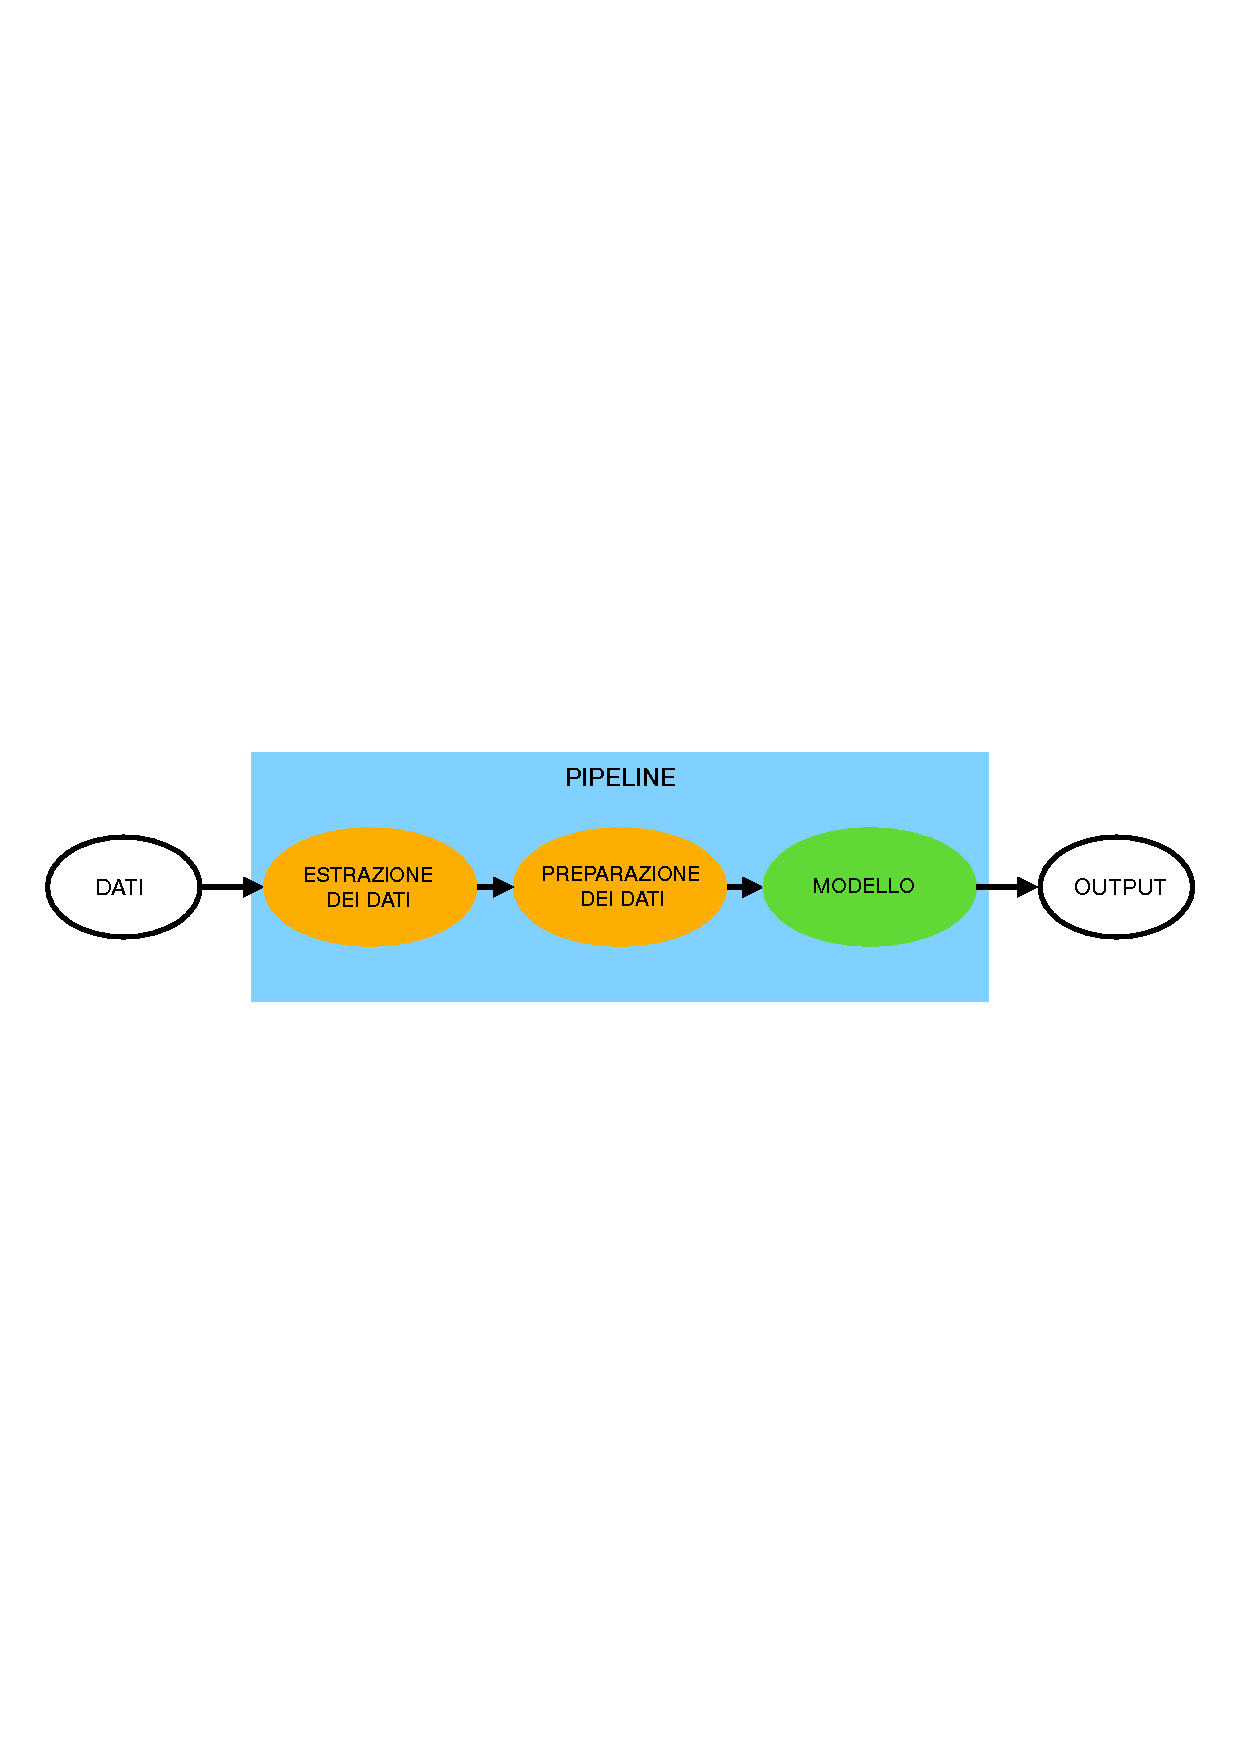
\includegraphics[trim=0 12.5cm 0 12.5cm, clip, width=\linewidth]{pipeline}
    \caption{Rappresentazione di una pipeline di Machine Learning come un
    grafo orientato senza cicli}
    \label{fig:ml_pipeline_dag}
\end{figure}

L'uso di una pipeline nel Machine Learning ci permette di ottenere i seguenti
vantaggi:
\begin{itemize}
    \item[\textit{Efficacia}] \textbf{Estensione della ricerca degli
        iperparametri ad altri componenti}: Mentre l'individuazione dei
        parametri ottimali per un modello avviene in modo automatico durante
        l'addestramento, la ricerca degli iperparametri migliori richiede
        sperimentazioni multiple, testando diversi valori e valutando i
        risultati del modello secondo metriche prestabilite. Dato che
        esternamente una pipeline funziona esattamente come un modello, è
        possibile estendere la ricerca degli iperparametri migliori a
        componenti non direttamente correlati al modello stesso, come quelle
        legate all'estrazione e alla preparazione dei dati. Poiché anche la
        ricerca degli iperparametri è automatizzabile, è possibile testare
        automaticamente diverse tecniche di preparazione dei dati,
        semplicemente integrando il componente alla pipeline, sebbene questo
        possa comportare un aumento del tempo di addestramento.
    \item [\textit{Efficienza}]\textbf{Sperimentazione rapida}:
        L'organizzazione di tutti i passaggi in una pipeline può accelerare
        notevolmente la sperimentazione. Questo è particolarmente utile quando
        si prevede di testare vari iperparametri o di utilizzare differenti
        sottoinsiemi di dati. Infatti, incapsulando le operazioni delle
        diverse componenti in un unico elemento che le esegue sequenzialmente,
        si evita di ripetere le stesse operazioni più volte, risultando in un
        risparmio di tempo significativo.
\end{itemize}

Nelle sezioni seguenti, descriveremo come sono stati affrontati i vari
passaggi nella creazione di un modello di Machine Learning per
l'identificazione dei job zombie e come si è cercato di integrare ciascun
componente alla pipeline.

\section{Estrazione dei dati}

L'estrazione di un dataset viene fatta tramite una query SQL che interroga le
tabelle \texttt{hj} e \texttt{htjob}, selezionando i dati rilevanti.
Ricordando che:
\begin{itemize}
    \item La tabella \texttt{hj} contiene lo stato dei job, rappresentato da
        serie storiche di misurazioni (come \texttt{runtime}, \texttt{ram},
        \texttt{swap}, \texttt{disk}, ecc.),
        durante la loro esecuzione.
    \item La tabella \texttt{htjob} fornisce informazioni sullo stato finale
        dei job, tra cui l'esito, indicando se sono falliti o meno.
\end{itemize}

La query esegue le seguenti operazioni:
\begin{itemize}
    \item Seleziona i job che hanno iniziato e finito la loro esecuzione nel
        periodo temporale specificato.
    \item Esegue un JOIN delle tabelle utilizzando l'identificativo univoco di
        ciascun job (\textit{jobid.idx\_submitnode}) e il timestamp. Questo
        timestamp sfrutta l'indice presente nella tabella \texttt{hj} per
        gestire in maniera efficiente le sue grandi dimensioni\footnote{La
            logica dietro questo consiste nel selezionare un job da
            \texttt{htjob} e successivamente cercarlo in \texttt{hj} limitando
            la ricerca ai record che rientrano nel periodo in cui
            \texttt{hj.ts} è compreso tra \texttt{htjob.starttimeepoch} e
            \texttt{htjob.eventtimeepoch}. Questo permette di restringere
            notevolmente la ricerca nella tabella \texttt{hj} per ogni job
            selezionato da \texttt{htjob} ed
        evitare di scansionare l'intera tabella.}. Poiché la tabella \texttt{hj} contiene più record per
        ogni job, la query li raggruppa per job. In seguito, mediante l'uso
        dell'operatore \verb|ARRAY_AGG|, le serie storiche vengono trasformate
        in array di valori.
    \item Seleziona i job con un tempo di esecuzione superiore a un'ora
        (\verb|runtime > 3600|), in quanto i job più brevi sono considerati
        irrilevanti per lo scopo dello studio.
\end{itemize}

Il risultato di questa query è un dataset come mostrato nella
figura~\ref{fig:dataset_from_join_hj_htjob}, dove ogni riga rappresenta un job
e le colonne includono: 

\begin{itemize}
    \item \texttt{job}: identificativo univoco per ogni job.
    \item \texttt{queue}: gruppo di appartenenza dell'utente che ha sottomesso
        il job.
    \item \texttt{fail}: un valore booleano che indica se il job è fallito.
    \item \texttt{mint} e \texttt{maxt}: Timestamp UNIX del momento in cui il
        job è stato eseguito e del momento in cui è terminato.
    \item \texttt{t}, \texttt{ram}, \texttt{swap}, \texttt{disk}: array di
        valori che rappresentano le serie storiche di misurazioni.
\end{itemize}

\begin{figure}[!ht]
    \centering
    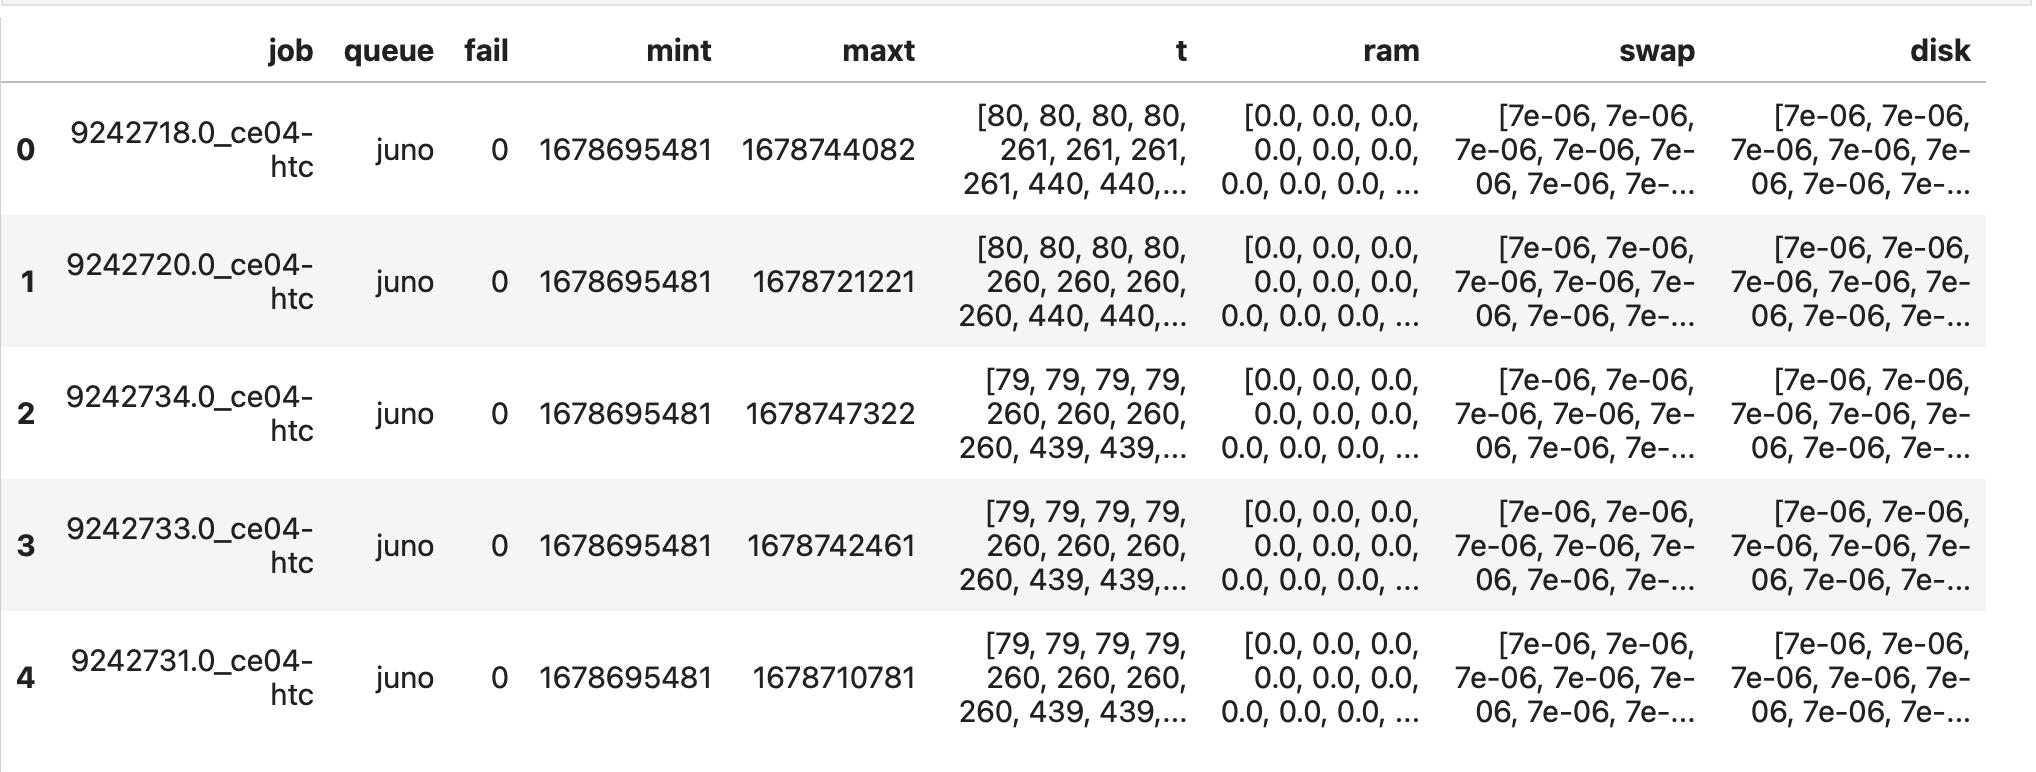
\includegraphics[width=0.95\textwidth]{dataset}
    \caption{Le prime cinque righe del dataset}
    \label{fig:dataset_from_join_hj_htjob}
\end{figure}

Tuttavia, il dataset estratto non è ancora pronto per l'addestramento del
modello e necessita di ulteriori trasformazioni da parte del componente
successivo. Questo passaggio non è stato integrato nella pipeline, in quanto,
nell'ambiente operativo reale, si prevede che questa lavori direttamente con i
dati forniti da HTCondor, eliminando così la necessità di estrarre dati da un
database SQL.

\section{Preparazione dei dati}
\label{sec:preprocessing}

La preparazione dei dati è essenziale nel Machine Learning. Prima di tutto, è
necessario convertire i dati disponibili in formato numerico, dato che gli
algoritmi di Machine Learning lavorano esclusivamente con dati in tale forma.
Inoltre, la qualità e la quantità dei dati sono determinanti per l'efficacia
del modello. Se i dati disponibili sono insufficienti o di bassa qualità, i
risultati saranno scadenti a prescindere dalla complessità del modello
utilizzato. Tipicamente, maggiore è la complessità di un modello, tanto più
esso richiederà una grande quantità di dati.

Per realizzare ciò, è stata creata una classe denominata
\texttt{Preprocessor}, che riceve in input un dataset e restituisce in output
un dataset modificato, eseguendo una serie di operazioni intermedie. Queste
operazioni possono essere ricondotte a tre categorie: l'aggiunta, la rimozione
e la trasformazione di colonne. Le operazioni effettuate sono configurabili
attraverso parametri definiti nel costruttore della classe al momento della
sua istanziazione. Quando questo componente viene inserito all'interno di una
pipeline, tali parametri fungono da iperparametri, permettendo di esplorare
diverse configurazioni per identificare quale produca i risultati migliori.

In aggiunta, questa classe è stata implementata seguendo il design pattern
Template Method \cite{gamma1994}, nel quale i passaggi di un algoritmo vengono
divisi in metodi separati, e successivamente invocati da un metodo denominato
template (vedi figura~\ref{fig:uml_preprocessor}). La superclasse definisce lo
scheletro dell'algoritmo, consentendo alle sottoclassi di personalizzare
alcuni passaggi sovrascrivendo alcuni metodi. In questo modo, è possibile
codificare la parte invariante dell'algoritmo una sola volta nella
superclasse, lasciando alle sottoclassi il compito di implementare i
comportamenti che possono variare. In pratica, l'uso di questo pattern in
questa classe ci consente di aggiungere, modificare e rimuovere passaggi
dall'algoritmo in modo semplice ed immediato, senza la necessità di dover
intervenire sul codice della classe principale.

\begin{figure}[!ht]
   \centering
   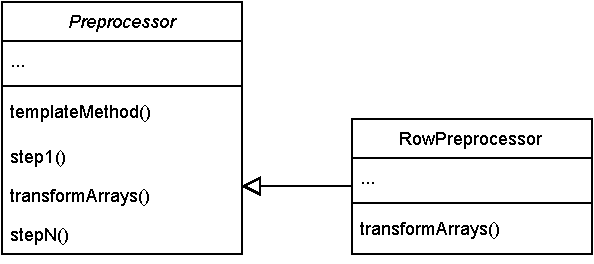
\includegraphics[width=0.5\linewidth]{preprocessor}
   \caption{Diagramma UML della classe \texttt{Preprocessor}, illustrante
   l'implementazione del design pattern Template Method}
   \label{fig:uml_preprocessor}
\end{figure}

Dopo aver delineato la struttura generale della classe \texttt{Preprocessor},
descriveremo ora le trasformazioni effettuate dal metodo
\texttt{preprocess()}, che funge da metodo template, nella preparazione dei
dati.

\subsection{Preparazione delle serie storiche}

Nella sezione~\ref{sec:job_analysis}, abbiamo identificato alcuni problemi
nelle misurazioni registrate da HTCondor relative allo stato dei job. Un
problema è la presenza di valori ripetuti all'interno delle serie storiche.
Queste serie sono attualmente rappresentate come array di valori, che non
corrispondono al formato numerico richiesto dai modelli di Machine Learning.
Pertanto, è necessario non solo rimuovere le ripetizioni, ma anche convertire
queste serie storiche in un formato di dati strutturato.

\paragraph{Riduzione della frequenza di campionamento.} Applicando
un'operazione di convoluzione\footnote{La convoluzione è una operazione
    matematica che consiste nell'applicare un filtro di dimensione finita
    lungo una sequenza di valori. Il filtro, di solito di piccole dimensioni,
    viene fatto scorrere su tutta la sequenza, e in ogni posizione si calcola
    una somma pesata tra i valori della sequenza e quelli del filtro. Questo
    processo trasforma la sequenza originale in una nuova attraverso la
formula: $$(S\ast K)(i)=\displaystyle\sum_{m=0}^{n}S(m)\cdot K(i-m)$$ dove
$S$ è la sequenza originale, $K$ è il filtro e $n$ è la dimensione del
filtro.} con un passo (\textit{stride}) di 5 e un filtro di 5 elementi con
valore $\frac{1}{5}$, possiamo effettuare una decimazione della sequenza
originale. Ciò comporta di ottenere una nuova sequenza, la cui lunghezza è
pari a un quinto della lunghezza della serie storica originale. In pratica, il
filtro calcola la media di ogni gruppo di cinque valori consecutivi. Se questi
cinque valori sono identici, il risultato sarà il valore stesso, che
sostituisce la sequenza dei cinque valori, eliminando le ripetizioni nella
nuova sequenza.

\paragraph{Trasformazione delle multiple serie storiche multivariate.} Sebbene
durante il processo di estrazione dei dati le serie storiche multivariate
siano state rappresentate come array, il dataset rappresenta ancora le tre
dimensioni delle multiple serie multivariate: job (righe), variabili (colonne)
e time step (array), come illustrato nella
figura~\ref{fig:multiple_multivariate_time-series}. Una possibile soluzione
potrebbe essere quella di trasformare gli array in una singola statistica,
come la media o il massimo, ma ciò cancellerebbe qualsiasi indicazione
sull'evoluzione temporale di ciascun job. Il nostro obiettivo è quello di
introdurre nuove feature che possano riflettere la tridimensionalità originale
dei dati. Tuttavia, prima di procedere, è necessario assicurarsi che tutte le
serie storiche siano uniformate alla stessa lunghezza.

\begin{figure}[!ht]
   \centering
   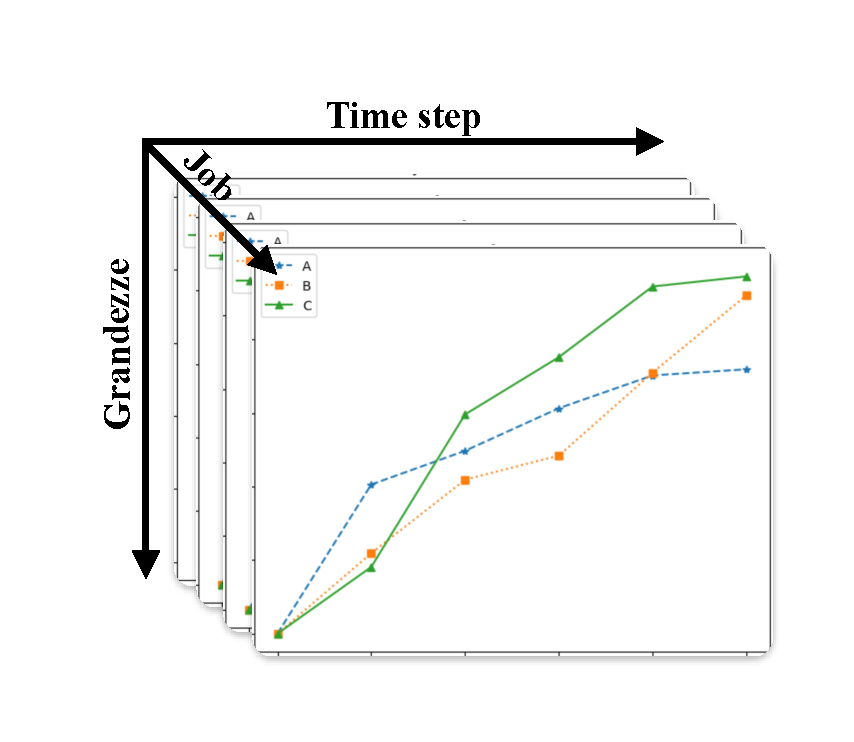
\includegraphics[trim=0cm 1.5cm 0cm 1.5cm, clip, width=0.5\linewidth]{multiple_multivariate_time-series}
   \caption{Rappresentazione tridimensionale delle multiple serie storiche
   multivariate}
   \label{fig:multiple_multivariate_time-series}
\end{figure}

Per gestire serie di dati con lunghezze diverse, possiamo utilizzare due
strategie: lo zero-padding e il troncamento. Lo zero-padding si applica alle
sequenze più corte, aggiungendo zeri fino a raggiungere una lunghezza
prefissata. Il troncamento, invece, si usa per ridurre le sequenze più lunghe,
tagliandole fino a che non raggiungono la stessa lunghezza prestabilita. La
classe \texttt{Preprocessor} implementa entrambe le tecniche: stabilisce una
lunghezza fissa per tutte le sequenze, troncando quelle che eccedono questa
lunghezza e applicando lo zero-padding a quelle che non la raggiungono.

Una volta ottenute serie storiche di uguale lunghezza, vengono applicate le
seguenti trasformazioni, in base al modello utilizzato:

\begin{itemize}
    \item \textbf{Trasformazione in colonne}: Ogni elemento di ogni array
        diventa una colonna (feature) separata nel dataset. Ad esempio, con un
        sottocampionamento a 15 minuti per un giorno, avremo 96 time step,
        corrispondenti a 96 colonne per ciascuna serie temporale.
    \item \textbf{Trasformazione in righe}: Gli elementi nelle stesse
        posizioni negli array formano righe distinte. Quindi, con un
        sottocampionamento a 15 minuti per un giorno, otteniamo 96 righe per
        ogni job.
\end{itemize}

\subsection{Creazione delle feature}

Dopo aver convertito le serie storiche in formato numerico, rimangono alcune
colonne, come \texttt{job} e \texttt{queue}, che sono di tipo categorico
nominale e che necessitano anch'esse di essere convertite in formato numerico.
Inoltre, è importante assicurarsi che le colonne numeriche siano sulla stessa
scala, poiché le differenze di scala possono portare a prestazioni subottimali
nei modelli. Quindi, un passo importante nella preparazione dei dati è il
ridimensionamento di queste colonne.

\paragraph{One-hot encoding.} 
\label{par:features}

Una possibile soluzione per gestire le colonne di tipo categorico potrebbe
essere quella di assegnare un valore intero a ciascun valore categorico.
Tuttavia, questa strategia può indurre il modello a interpretare i valori
numerici vicini come simili e quelli distanti come dissimili, il che non è
appropriato per le colonne di tipo categorico nominale.

Per risolvere questo problema, si può utilizzare la tecnica dell'one-hot
encoding, che crea una colonna binaria per ogni valore categorico: la colonna
sarà impostata a 1 per la categoria corrispondente e a 0 per tutte le altre.
Sfortunatamente, il one-hot encoding può generare un eccessivo numero di
colonne in presenza di colonne con alta cardinalità, come \texttt{job}
($\mathcal{O}(\text{numero righe})$) o \texttt{queue} ($\mathcal{O}(50)$). In
questi casi, si rischia di avere troppe feature irrilevanti, compromettendo
l'efficacia del modello di Machine Learning. 

Per garantire che il modello impari efficacemente dai dati, è fondamentale
selezionare feature rilevanti ed eliminare quelle irrilevanti. È altresì
importante che il modello interpreti i dati in modo simile a come li
percepiamo noi, evidenziando le caratteristiche salienti dei dati e la
struttura del problema. 

Per far ciò, sono state create due nuove colonne, \texttt{job type} e
\texttt{job work type} (vedi figura~\ref{fig:job_type_and_job_work_type}),
seguite dall'applicazione dell'one-hot encoding. La prima colonna raggruppa i
gruppi di utenti, in LHC e non-LHC, che, come osservato nell'analisi
preliminare, hanno meccanismi interni diversi e potrebbero comportarsi in
maniera differente. Allo stesso modo, viene estratto il \verb|submit_node|
dalla colonna \texttt{job}, dove ogni ID è composto da
\verb|jobid.idx_submitnode|, e classificato i job in base al fatto che il
\verb|submit_node| sia ``sn0x'' o ``ce0x'', distinguendo così i job sottomessi
dagli utenti interni del CNAF da quelli degli utenti esterni.

\begin{figure}[!ht]
    \centering
    \begin{tikzpicture}[sibling distance=2cm]
        \node {JOB TYPE}
        child {node {GRID}}
        child {node {LOCAL}};
    \end{tikzpicture}
    \hspace{2cm}
    \begin{tikzpicture}[sibling distance=2cm]
        \node {JOB WORK TYPE}
        child {node {LHC}}
        child {node {NON-LHC}};
    \end{tikzpicture}
    \caption{Visualizzazione delle nuove colonne \texttt{job type} e \texttt{job work type}}
    \label{fig:job_type_and_job_work_type}
\end{figure}

\paragraph{Ridimensionamento delle feature.} Ridimensionare i dati è un passo
cruciale per migliorare la convergenza durante l'addestramento dei modelli
\cite{LeCun2012}. Questo passaggio è essenziale per alcuni di questi, come le
reti neurali, dove il ridimensionamento dei dati è una precondizione. Al
contrario, altri modelli, quali gli alberi decisionali, non richiedono
specifiche assunzioni sui dati.

Sono state utilizzate due tecniche di ridimensionamento: la normalizzazione e
la standardizzazione. La normalizzazione è il processo che ridimensiona i dati
in un intervallo tra 0 e 1. La formula è
$X'=\frac{(X-X_{\min})}{X_{\max}-X_{\min}}$, dove $X_{\min}$ e $X_{\max}$ sono
rispettivamente i valori minimi e massimi della feature. La standardizzazione
trasforma i dati in modo che abbiano media 0 e varianza di 1. La formula è
$X'=\frac{X-\mu}{\sigma}$ dove $\mu$ è la media e $\sigma$ la deviazione
standard.

La decisione di quale tecnica utilizzare dipende dalla specifica natura del
problema affrontato, in quanto diversi problemi possono beneficiare di diverse
tecniche di ridimensionamento. In pratica, andremo a testare entrambe le
tecniche per determinare quale funziona meglio con il modello in uso.

\subsection{Etichettatura dei dati}

In base alla presenza di etichette nei dati, possiamo distinguere tra
apprendimento supervisionato e non supervisionato. Nell'apprendimento
supervisionato, i modelli vengono addestrati con un dataset, dove ogni esempio
è associato a un'etichetta, rappresentante un valore categorico o numerico.
Durante l'addestramento, il modello tenta di prevedere le etichette per esempi
che non ha mai visto prima. Le predizioni sono poi confrontate con le
etichette per calcolare l'errore, che indica quanto le predizioni del modello
si discostano dai valori reali. L'obiettivo è migliorare la precisione del
modello minimizzando l'errore della funzione costo, tipicamente attraverso la
discesa del gradiente.

Attualmente, il dataset non include etichette che identifichino quali job
siano zombie, il che ci impedisce di impostare un apprendimento
supervisionato. Per generare le etichette, calcoliamo il tempo di esecuzione
di ogni job come \verb|int((maxt - mint) / 86400)| per ottenere il numero di
giorni di esecuzione. Poi, con la colonna \texttt{job\_type}, etichettiamo
come job zombie quelli che vengono rimossi dal batch system dopo aver superato
il massimo tempo di esecuzione, cioè 3 giorni per i job grid, e 7 per quelli
locali.

\subsection{Tecniche di bilanciamento dei dati}
\label{sec:imbalanced_data}

Nella sezione~\ref{sec:job_analysis}, abbiamo osservato che i job zombie sono
estremamente più rari dei job normali, con un rapporto di 1 a 10,000. A causa
di questo forte sbilanciamento, il classificatore potrebbe semplicemente
apprendere a identificare tutti gli esempi come job normali (etichettati come
0), ottenendo così un errore apparentemente molto basso, ma in realtà
ignorando completamente i job zombie, che sono esattamente quelli che
desideriamo identificare. 

Per tentare di ridurre il bias del modello verso la classe maggioritaria sono
state adottate tre tecniche in combinazione: sottocampionamento,
sovracampionamento e Cost-sensitive learning. Queste tecniche mirano a
bilanciare la distribuzione delle classi nel dataset e a migliorare la
capacità del modello di distinguere tra job normali e job zombie. 

\paragraph{Sottocampionamento casuale.} Il sottocampionamento casuale è una
strategia molto semplice in cui vengono cancellati casualmente degli esempi di
job normali dal dataset. Tuttavia, ciò può comportare la perdita di
informazioni preziose per il modello, causando una perdita della sua
precisione \cite{he2013}.

\paragraph{Sovracampionamento.}
\label{par:vae}

Un'alternativa è il sovracampionamento dei job zombie. Il metodo più semplice
consiste nell'aggiungere duplicati di esempi già presenti nel dataset;
tuttavia, ciò non fornisce nuove informazioni utili al modello. Un approccio
più efficace è la generazioni di nuovi esempi artificiali, che sono varianti
dei job zombie \cite{brownlee2021}. 

Pertanto, si è scelto di usare una variante dell'autoencoder, nota come
\textbf{variational autoencoder} \cite{kingma2022}, per generare varianti di
job zombie a partire dai job zombie dell'intero 2021. Gli autoencoder
tradizionali apprendono funzioni per mappare esempi in punti nello spazio
latente e viceversa, per mappare le loro rappresentazioni compresse dallo
spazio latente allo spazio originale. Tuttavia, se si prende una variante di
un esempio nello spazio latente, il decoder $g(h)$ genererà un output privo di
senso, in quanto non è in grado di gestire regioni dello spazio mai esplorate.
Il variational autoencoder risolve questo problema facendo sì che l'encoder
anziché restituire una rappresentazione compressa $h$, fornisca una media
$\mu$ e una deviazione standard $\sigma$. Intuitivamente, la rappresentazione
compressa viene campionata da una distribuzione gaussiana caratterizzata dalla
media $\mu$ e dalla deviazione standard $\sigma$. In questo modo, il decoder
impara a mappare non solo un singolo punto nello spazio latente, ma anche
tutti i punti nelle sue vicinanze (vedi figura~\ref{fig:vae_comparison})
\cite{shafkat2018}.

Tuttavia, il sovracampionamento aumenta il rischio di overfitting, cioè la
possibilità che il modello si adatti eccessivamente ai dati di addestramento,
perdendo così la capacità di generalizzare su dati nuovi \cite{fernandez2018}.

\begin{figure}
    \centering
    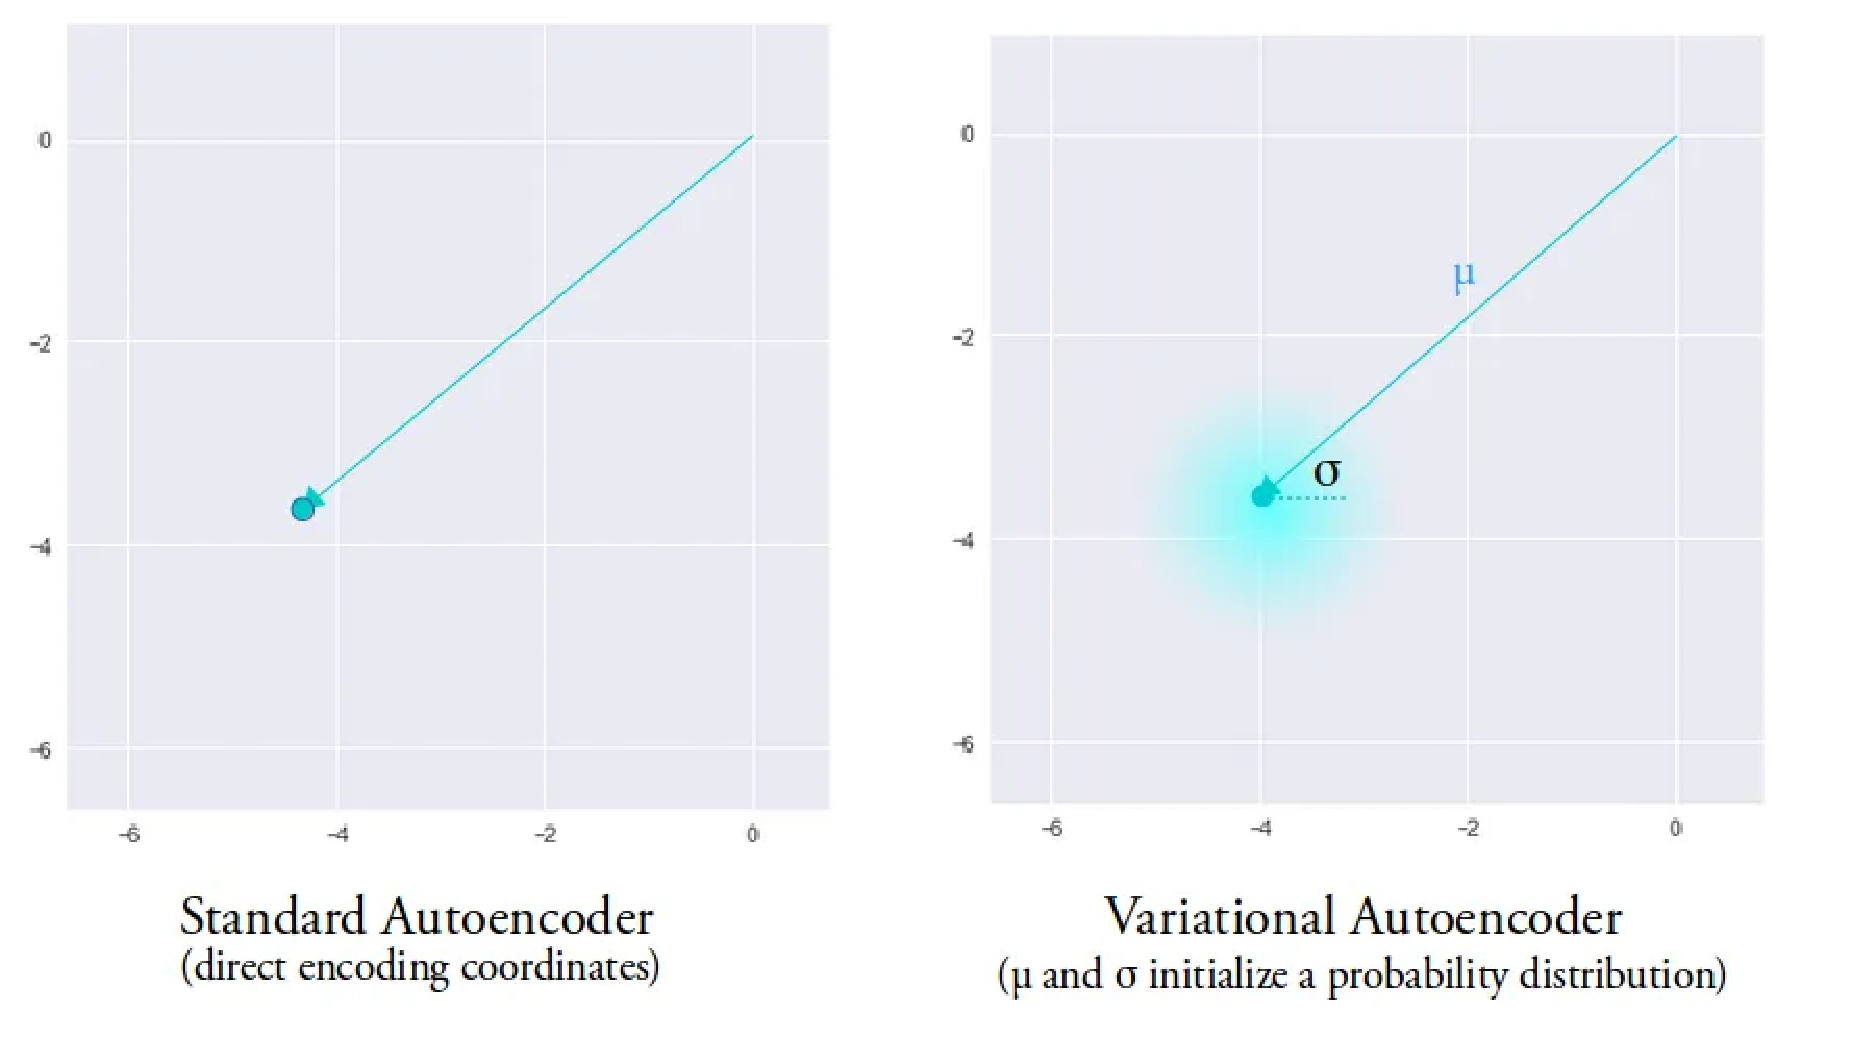
\includegraphics[width=0.95\linewidth]{vae_comparison}
    \caption{Rappresentazioni compresse in un autoencoder tradizionale e un
    variational autoencoder \cite{shafkat2018}}
    \label{fig:vae_comparison}
\end{figure}

\paragraph{Cost-sensitive learning.}

Possiamo distinguere gli errori commessi dal modello in falsi positivi e falsi
negativi in base a due criteri: un errore è falso positivo quando il modello
identifica erroneamente un job come zombie nonostante non lo sia; è invece un
falso negativo quando il modello etichetta come normale un job che in realtà è
zombie.

Assegnando un valore diverso, che definiamo ``costo'', ai falsi positivi e ai
falsi negativi, e minimizzando il costo totale\footnote{$\text{Costo totale} =
    C_{FN} \cdot
FN + C_{FP} \cdot FP$} derivante dalle predizioni
errate, il modello imparerà durante l'addestramento ad attribuire diversa
importanza ai vari tipi di errori.

\section{Selezioni dei modelli}
\label{sec:novelty_detection}

Nel Machine Learning, il problema di identificare i job zombie può essere
risolto modellando il problema in diversi modi e creando modelli specifici per
risolverlo. In questa tesi, si è scelto di approcciare il problema
modellandolo in due modi: la classificazione e la novelty detection.

Nel primo caso, al modello viene richiesto di specificare, come output, a
quale dei $k$ valori categorici un esempio appartiene. Per risolvere questo
problema, il modello deve produrre una funzione del tipo
$f:\mathbb{R}^n\to\{1,\ldots,k\}$ basandosi sulle feature degli esempi in
input \cite{Goodfellow2016}.

Nel caso della novelty detection, invece, si chiede al modello di modellare i
dati e di riconoscere le ``novità'', ovvero ciò che non ha mai visto dai dati.
Consideriamo una novità come un punto dei dati che non appare consistente con
ciò che è stato osservato nei dati di addestramento. A differenza della
classificazione, i  modelli non modellano esplicitamente un'anomalia; essi
imparano solo a riconoscere ciò che è normale. Per funzionare efficacemente,
l'addestramento richiede un dataset ``pulito'', cioè privo di job zombie
\cite{geron2019, pimentel2014}.

L'ipotesi è che, modellando sufficienti dati, possiamo ottenere un modello che
ha già visto abbastanza per riconoscere i job zombie come novità rispetto a
ciò che ha appreso come normale (vedi figura~\ref{fig:anomaly_detection}).

\begin{figure}[!ht]
    \centering
    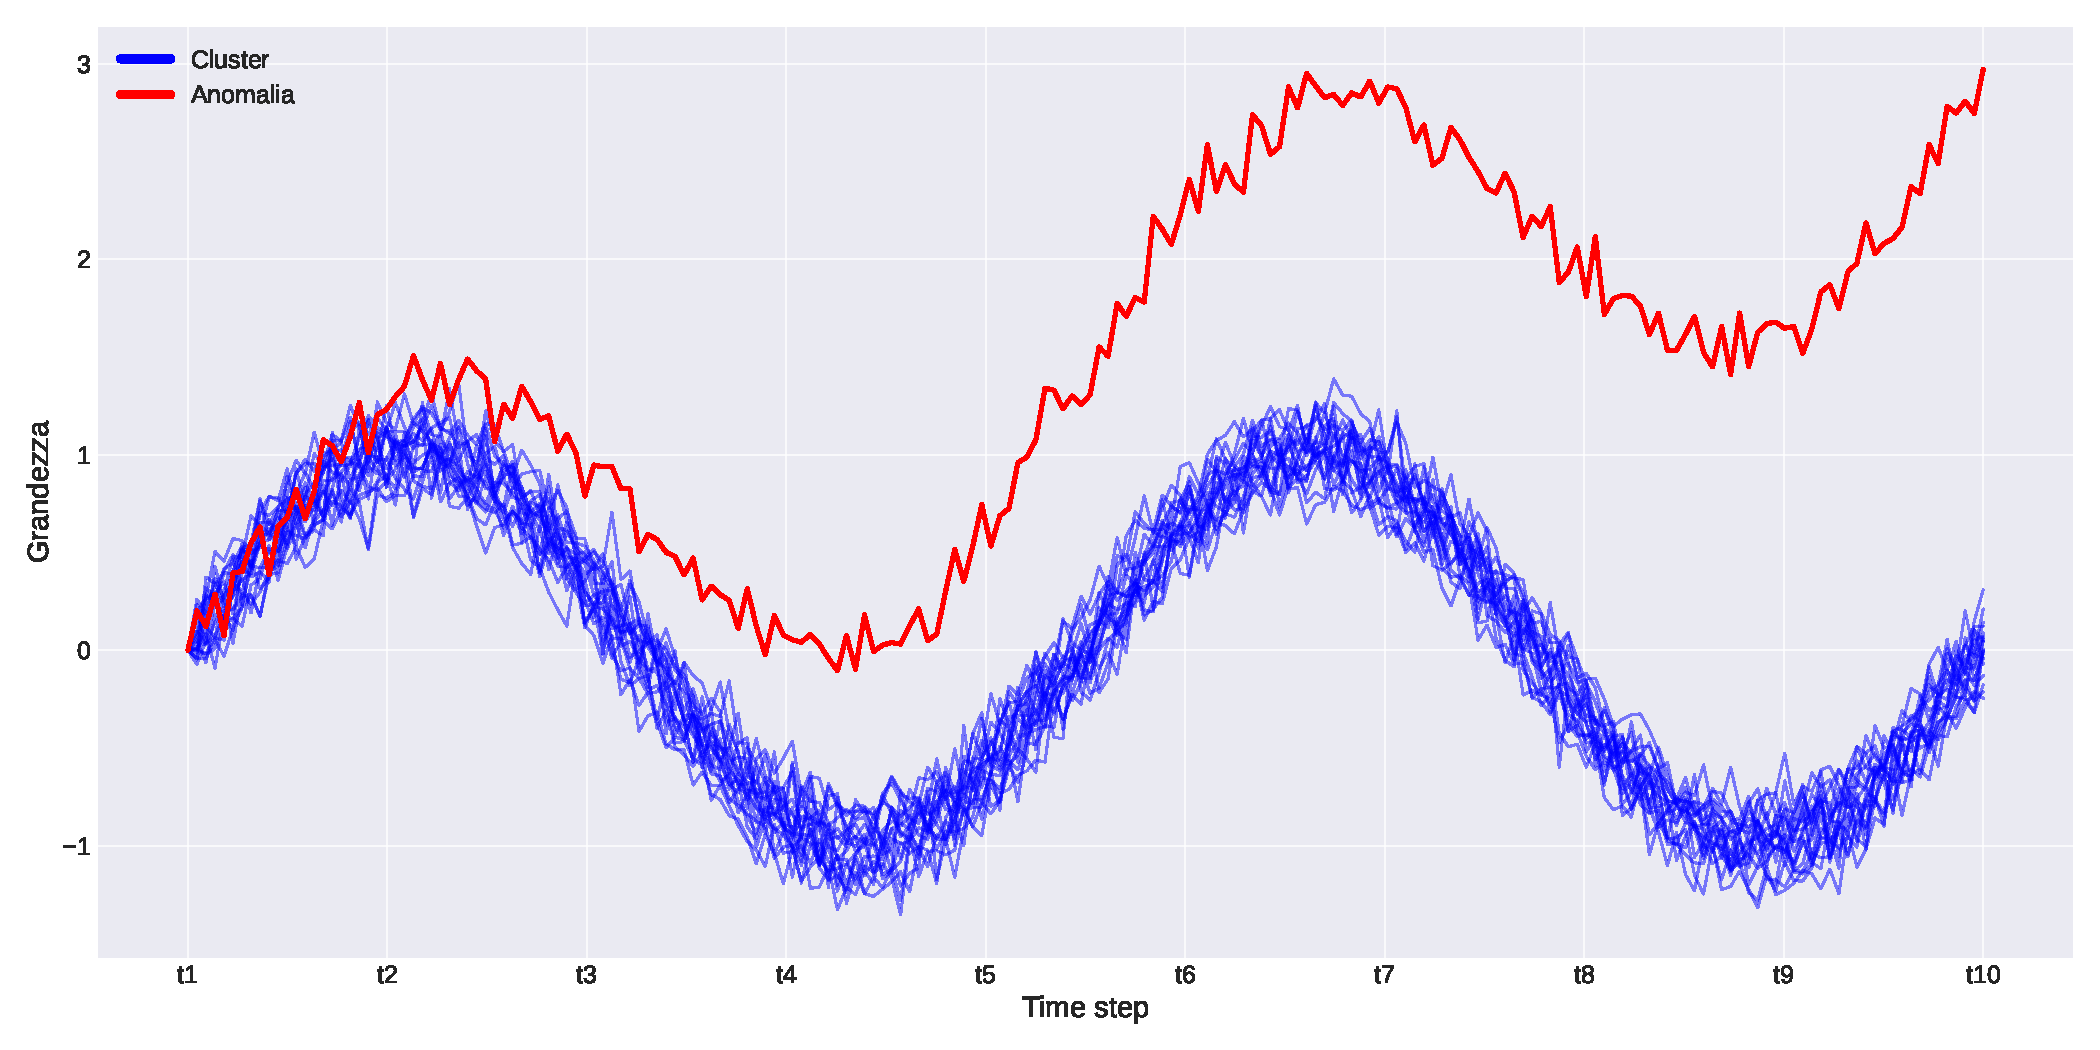
\includegraphics[width=0.95\linewidth]{anomaly_time_series}
    \caption{Rappresentazione ideale di una serie storica anomala in contrasto
    con un cluster di serie storiche normali}
    \label{fig:anomaly_detection}
\end{figure}

Procederemo con la presentazione dei modelli impiegati e illustreremo le
ragioni della loro scelta.

\subsection{XGBoost (Classificatore)}

XGBoost (eXtreme Gradient Boosting) è un modello basato su un insieme, o
``ensemble'', di alberi decisionali (vedi figura~\ref{fig:xgboost}). Ogni
albero in questo ensemble è sua volta un modello, con nodi intermedi
dell'albero che pongono domande binarie sulle feature dei dati, dividendoli in
sottoinsiemi. Questo processo si ripete ricorsivamente in ciascun nodo fino a
raggiungere i nodi foglia, che rappresentano le classificazioni finali per le
istanze.

XGBoost utilizza il metodo del Gradient Boosting per costruire l'ensemble di
alberi decisionali, mirando a combinare modelli ``deboli'' per formare un
modello ``forte''. In questo metodo, nuovi alberi decisionali vengono aggiunti
iterativamente, ciascuno addestrato per correggere gli errori residui del
precedente. Idealmente, aggiungendo sufficienti alberi, i residui si
distribuiranno casualmente attorno allo zero, rendendo impossibile ulteriori
distinzioni \cite{breiman1997, friedman2001}.

In pratica, il processo inizia con un modello che fa previsioni costanti (per
esempio, predice sempre 0) e, ad ogni iterazione $k$, viene aggiunto un nuovo
modello $\hat{y}_i^{(k)}=f_k(x_i)$ al precedente fino al raggiungimento del
numero massimo di alberi definito da un iperparametro. La struttura di questo
processo può essere descritto dalle seguenti equazioni:

\begin{center}
    \begin{math}
        \begin{aligned}
            \hat{y}^{(0)} &=0 \\ 
            \hat{y}^{(1)}&=f_1(x_i)=\hat{y}_i^{(0)}+f_1(x_i)\\ 
            \vdots \\ 
            \hat{y}_i^{(t)}&=\sum_{k=1}^{t}f_k=\hat{y}_i^{(t-1)}+f_t(x_i)
        \end{aligned}
    \end{math}
\end{center}

L'ensemble può essere rappresentato come la somma di $t$ funzioni,
$\sum_{k=1}^{t}f_k(x_i)$, dove ogni funzione corrisponde a un albero. Durante
l'addestramento, XGBoost ottimizza queste $t$ funzioni con la seguente
funzione obiettivo\footnote{La funzione che andremo a minimizzare durante
l'addestramento.}:

$$\text{obj}^{(t)}=\displaystyle\sum_{i=1}^{n}\ell(y_i,\hat{y}_i^{(t)})+\displaystyle\sum_{k=1}^{t}\Omega(f_k)$$

che è la somma delle funzioni di perdita\footnote{La funzione di perdita
misura la discrepanza tra i valori predetti dal modello e i valori reali dei
dati.} e dei termini di regolarizzazione per i $t$ alberi. Il termine di
regolarizzazione, introdotto da XGBoost come ottimizzazione al Gradient
Boosting insieme ad altre ottimizzazioni, contribuisce a ridurre il rischio di
overfitting \cite{chen2016}. 

Una volta che il modello è addestrato, le predizioni vengono effettuate
calcolando le predizione di ogni albero e sommando insieme i risultati di
tutti gli alberi per ottenere la previsione finale.

\begin{figure}[!ht]
    \centering
    \includegraphics[page=6,trim=4.5cm 16.5cm 4.5cm 5.5cm, clip, width=0.9\linewidth]{xgboost}
    \caption{Struttura semplificata di XGBoost \protect\cite{guo2020}}
    \label{fig:xgboost}
\end{figure}

Nonostante il teorema ``no free lunch'' affermi che non esista un modello che
a priori sia superiore ad altri e che la scelta del modello possa essere
determinata solo attraverso test comparativi, XGBoost si tratta di un'ottima
prima scelta nella trattazione di problemi reali, grazie alla sua efficacia
nel trattare dati strutturati \cite{shwartz2021, chen2016}.

\subsection{Reti neurali (Classificatore)}
\label{sec:nn}

Come discusso nel paragrafo~\ref{par:features}, la creazione di un modello che
apprenda efficacemente dai dati richiede un'attenta selezione di feature
rilevanti, un processo che non è semplice. Un'alternativa è l'uso di reti
neurale profonde per la classificazione. Le reti neurali convoluzionali (CNN),
ad esempio, offrono il vantaggio di estrarre automaticamente le feature più
rilevanti durante l'addestramento. Altre tipi di reti, come le reti neurali
ricorrenti (RNN) e i Transformer, sono in grado di utilizzare l'intera storia
di una serie temporale e catturare le dipendenze temporali per fare delle
previsioni.

Una rete neurale è composta da unità chiamate neuroni, organizzati in strati:
uno strato di input, che riceve i dati iniziali; uno o più strati nascosti che
elaborano i dati; e infine uno strato di output, che produce il risultato
finale. I neuroni di ogni strato sono connessi a quelli degli strati adiacenti
tramite connessioni pesate (vedi figura~\ref{fig:neural_network}).

\begin{figure}[!ht]
    \centering
    \begin{neuralnetwork}[height=4]
        \newcommand{\nodetextclear}[2]{}
        \newcommand{\nodetextx}[2]{$x_#2$}
        \newcommand{\nodetexty}[2]{$y_#2$}
        \inputlayer[count=3, bias=false, title=Input\\layer, text=\nodetextx]
        \hiddenlayer[count=4, bias=false, title=Hidden\\layer, text=\nodetextclear] \linklayers
        \outputlayer[count=2, title=Output\\layer, text=\nodetexty] \linklayers
    \end{neuralnetwork}
    \caption{Struttura di una rete neurale con uno strato nascosto} 
    \label{fig:neural_network}
\end{figure}

In ogni strato, ciascun neurone riceve input da altri neuroni o dall'esterno,
elabora questi input per produrre un output, che viene restituito ad altri
neuroni o all'esterno. Come mostrato nella figura~\ref{fig:neuron}, il neurone
calcola l'output come la somma pesata dei suoi input, a cui si aggiunge un
bias e successivamente applica una funzione di attivazione, indicata con
$\sigma$. Matematicamente, per il $j$-esimo neurone, l'output $y_j$ può essere
espresso come:

$$y_j=\sigma(\displaystyle\sum_{i}w_{j,i}\cdot x_i+b_j)$$

\begin{figure}[!ht]
    \centering
    \begin{neuralnetwork}[height=4]
        \newcommand{\nodetextclear}[2]{$\Sigma | \sigma$}
        \newcommand{\nodetextx}[2]{\ifthenelse{\equal{#2}{0}}{$b$}{$x_{#2}$}}
        \newcommand{\nodetexty}[2]{$y$}
        \newcommand{\linktextw}[4]{$w_#2$}
        \inputlayer[count=3, top=true, bias=true, title=Inputs, text=\nodetextx] 
        \hiddenlayer[count=1, top=true, bias=false, text=\nodetextclear]
        \outputlayer[count=1, top=true, title=Output, text=\nodetexty] 
        \link[from layer=0, to layer=1, from node=0, to node=1]
        \link[from layer=0, to layer=1, from node=1, to node=1, label=\linktextw]
        \link[from layer=0, to layer=1, from node=2, to node=1, label=\linktextw]
        \link[from layer=0, to layer=1, from node=3, to node=1, label=\linktextw]
        \link[from layer=1, to layer=2, from node=1, to node=1]
    \end{neuralnetwork}
    \caption{Struttura di un neurone}
    \label{fig:neuron}
\end{figure}

Dove i pesi $w_{j,i}$ per ciascun input $x_i$ e il bias $b_j$ sono i parametri
del neurone. Considerando tutti i neuroni, questi sono i parametri complessivi
della rete. I pesi vengono inizializzati in modo semi-casuale e, durante
l'addestramento, si procede a regolare i parametri della rete per ottenere
l'output desiderato.

\subsubsection{Reti neurali convoluzionali}

Nelle reti neurali, il modo in cui i neuroni sono connessi permette di
eseguire diverse operazioni. Quando ogni neurone di uno strato è collegato a
tutti quelli degli strati adiacenti, si parla di strati densi. Nelle reti
convoluzionali, invece, i neuroni di uno strato sono connessi solamente a un
sottoinsieme di quelli dello strato precedente, generalmente vicini (vedi
figura~\ref{fig:convnet}).

\begin{figure}[!ht]
    \centering
    \begin{neuralnetwork}[height=4]
        \newcommand{\nodetextclear}[2]{}
        \hiddenlayer[count=4, bias=false,  text=\nodetextclear]        
        \hiddenlayer[count=4, bias=false,  text=\nodetextclear] 
        \link[from layer=0, to layer=1, from node=1, to node=1]
        \link[from layer=0, to layer=1, from node=2, to node=2]
        \link[from layer=0, to layer=1, from node=3, to node=3]
        \link[from layer=0, to layer=1, from node=4, to node=4]

        \link[from layer=0, to layer=1, from node=1, to node=2]
        \link[from layer=0, to layer=1, from node=2, to node=3]
        \link[from layer=0, to layer=1, from node=3, to node=4]

        \link[from layer=0, to layer=1, from node=4, to node=3]
        \link[from layer=0, to layer=1, from node=3, to node=2]
        \link[from layer=0, to layer=1, from node=2, to node=1]
    \end{neuralnetwork}
    \caption{Visualizzazione delle connessioni tra i neuroni in uno strato
    convoluzionale} 
    \label{fig:convnet}
\end{figure}

Quest'operazione è equivalente a una convoluzione, dove un filtro (o feature
detector) scorre attraverso l'input, con i pesi del filtro che vengono appresi
durante l'addestramento. Ciò significa che, se i neuroni in uno strato
convoluzionale condividono lo stesso insieme di pesi, ciò equivale ad
applicare lo stesso filtro su tutti gli input. Gli output dei neuroni che
condividono gli stessi pesi forma una ``feature map''. Il filtro utilizzato
nella convoluzione corrisponde all'insieme dei pesi condivisi dai neuroni
all'interno di una feature map. Uno strato convoluzionale è composto da
molteplici feature map, ciascuna con un proprio insieme di pesi, in modo che
diverse feature possono essere estratte \cite{lecun1998}.

Questa struttura permette ai neuroni degli strati convoluzionali inferiori di
estrarre feature elementari, mentre gli strati successivi combinano queste
feature per ottenere rappresentazioni più complesse (vedi
figura~\ref{fig:feature_extractor}). 

\begin{figure}[!ht]
    \includegraphics[page=7, trim=3.5cm 3.5cm 3.5cm 22.5cm, clip, ,
    width=\linewidth]{feature_extractor}
    \caption{Estrazione delle feature da parte di una rete neurale convoluzionale \protect\cite{he2020}}
    \label{fig:feature_extractor}
\end{figure}

\subsubsection{Reti neurali ricorrenti e Transformers}

Le RNN hanno la capacità di ``ricordare'' la storia degli input processati in
uno stato, utilizzandola per elaborare nuovi input e produrre output. Questo
le rende particolarmente adatte per le serie temporali, dove eventi passati
potrebbero essere importanti per prevedere eventi futuri.

Come illustrato dalla figura~\ref{fig:rnn}, Una RNN può essere rappresentata
come un neurone che riceve un input, genera un output e poi riutilizza questo
output come input per il passo successivo. Le RNN lavorano con sequenze di
input (per esempio, $(x_{(0)}, x_{(1)},\ldots)$), dove ciascun elemento
corrisponde a un time step. Ad ogni time step $t$, il neurone riceve l'input
$x_{(t)}$ e l'output del time step precedente $y_{(t-1)}$ (se è il primo
input, riceve 0). Ogni neurone delle RNN ha due vettori di pesi: $W_x$ per gli
input $x_{(t)}$ e $W_y$ per gli output del time step precedente $y_{(t-1)}$.
L'output di ogni time step $y_{(t)}$ si calcola come
$y_{(t)}=\sigma_h(W_x\cdot x_{(t)}+W_y\cdot y_{(t-1)}+b)$ \cite{geron2019}.

\begin{figure}[!ht]
    \centering
    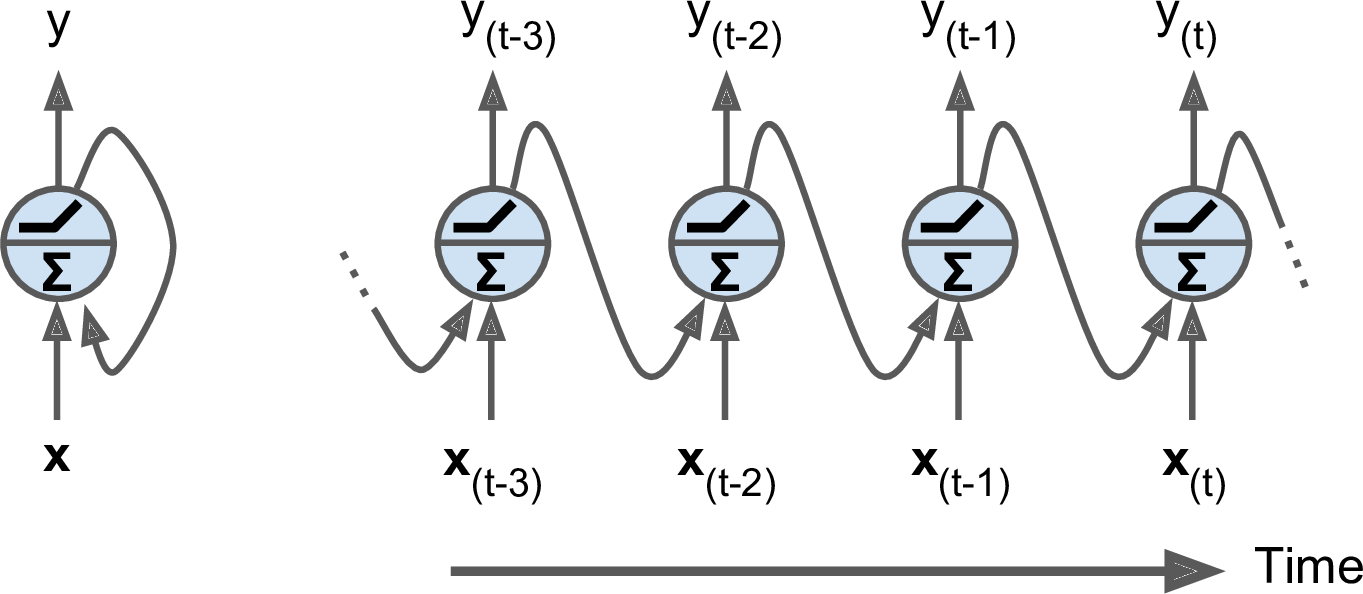
\includegraphics[width=0.75\linewidth]{rnn}
    \caption{Struttura di una semplice rete neurale ricorrente \protect\cite{geron2019}}
    \label{fig:rnn}
\end{figure}

Elaborata l'intera sequenza di input, lo stato della rete viene resettato.

Tuttavia, le RNN presentano un problema significativo: la loro capacità di
trattenere informazioni negli stati è limitata principalmente al time step
successivo. Ciò implica che l'influenza di un valore specifico nella sequenza
tende a svanire rapidamente, rendendo difficile catturare dipendenze a lungo
termine nelle serie temporali. Per ovviare a questo problema, sono stati
sviluppate varianti di RNN, come le Long Short-Term Memory (LSTM)
\cite{hochreiter1997} o altri tipi di reti neurali, quali i Transformer
\cite{vaswani2023}.

Il Transformer, diversamente delle RNN, processa l'intera sequenza in un unico
passaggio, apprendendo le relazioni tra i vari elementi della sequenza
attraverso i meccanismi del multi-head attention e il positional encoding. A
differenza delle RNN, che elaborano la sequenza un passo alla volta, il
Transformer non conosce l'ordine dei valori all'interno di essa. Di
conseguenza, è necessario incorporare tale ordine attraverso il positional
encoding. Il meccanismo di self attention, d'altra parte, estrae le relazioni
tra i valori nella sequenza, indipendentemente dalla loro distanza nella
sequenza, dando importanza ai valori più importanti nella sequenza.

\subsection{Autoencoder (Novelty detection)}
\label{sec:autoencoder}

Un autoencoder è anch'esso un modello che viene addestrato per minimizzare
l'errore di ricostruzione di un input dopo averlo compresso in uno spazio
latente. Durante l'addestramento con un dataset ``pulito'', l'encoder impara a
comprimere gli esempi nello spazio latente, mentre il decoder impara a
ricostruirli nella loro forma originale. Come visto nel
paragrafo~\ref{par:vae}, quando si fornisce al autoencoder esempi non visti in
fase di addestramento, se questi vengono compressi in qualcosa di simile a ciò
che ha già compresso nello spazio latente, allora riesce a ricostruire l'input
con buona fedeltà. In caso contrario, non riuscirà a costruire correttamente
l'input e l'errore di ricostruzione, definito come $\epsilon=\lVert
x-g(f(x))\rVert$, sarà alto \cite{borghesi2019}.

Per stabilire se un esempio è una novità, viene considerato l'errore di
ricostruzione insieme alle etichette. Utilizzando un secondo dataset che
comprende i job zombie, si imposta un valore soglia in base all'errore di
ricostruzione: quelli che sono sopra la soglia sono job zombie (1) e quelli
che sono al di sotto sono job normali (0) (vedi
figura~\ref{fig:reconstruction_error}). Minimizziamo il valore soglia per
avere un valore il più corretto possibile.

\begin{figure}[!ht]
    \centering
    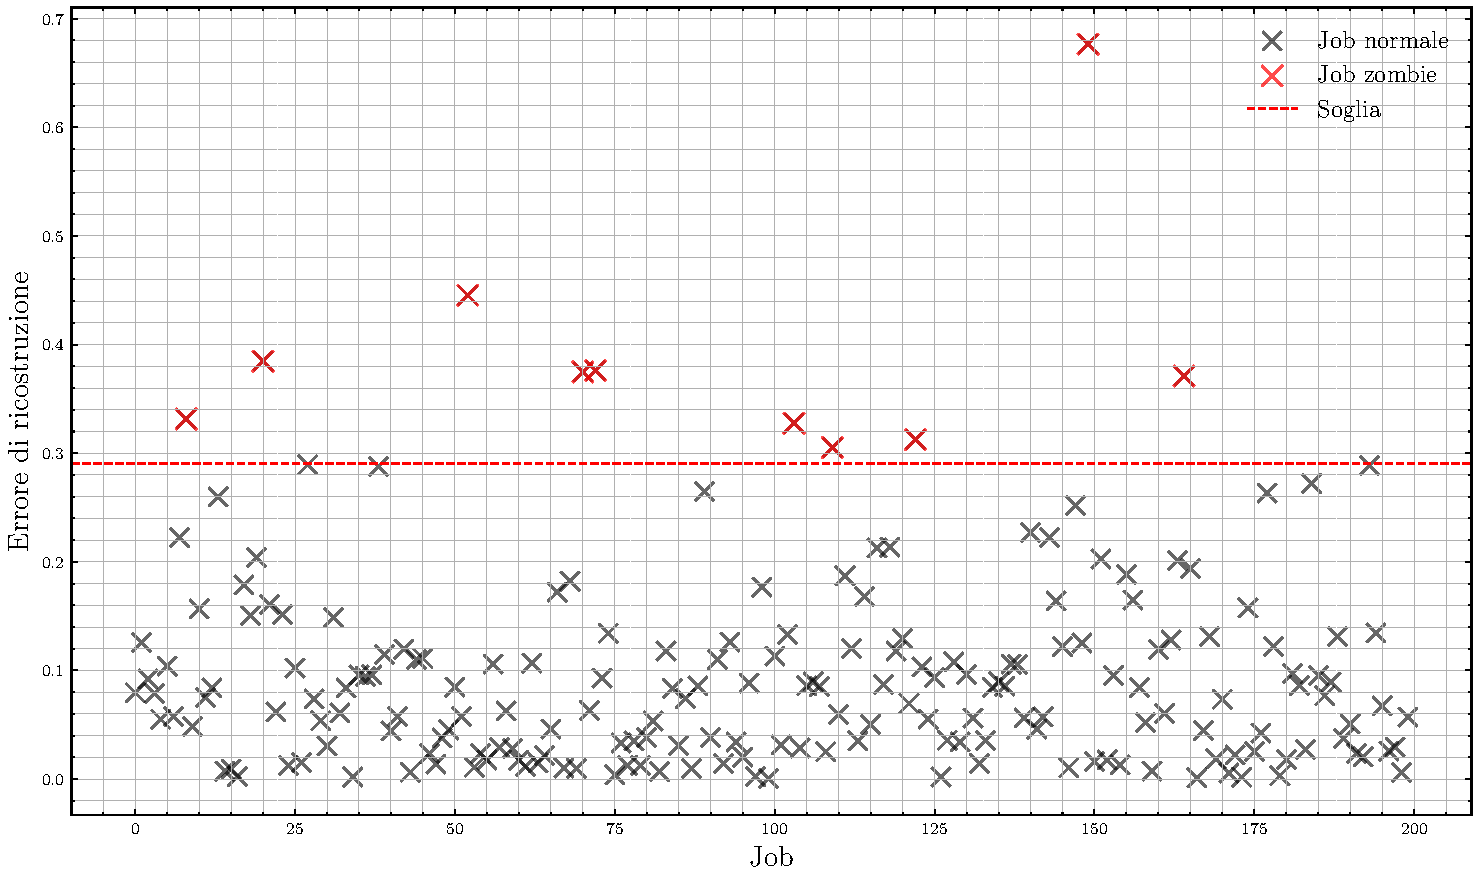
\includegraphics[width=0.85\linewidth]{reconstruction_error}
    \caption{Visualizzazione dell'errore di ricostruzione e della soglia per
    stabilire se gli esempi sono novità}
    \label{fig:reconstruction_error}
\end{figure}

Gli autoencoder, descritti finora in termini di funzioni encoder $f$ e decoder
$g$, sono costituiti da strati e neuroni. L'output dello strato intermedio
rappresenta la rappresentazione nello spazio latente. L'obiettivo è quello di
formare cluster efficaci in questo spazio latente, al fine di poter associare
nuovi job, mai incontrati prima, a gruppi di job esistenti. Tipicamente, per
questo scopo, gli autoencoder sono strutturati con una forma a clessidra (vedi
figura~\ref{fig:autoencoder}), o possono introdurre del rumore negli input,
oppure ancora aggiungere un termine di regolarizzazione alla funzione di
perdita per ``spegnere'' alcuni neuroni nello strato intermedio.

\begin{figure}[!hb]
    \centering 
    \begin{neuralnetwork}[height=4]
        \newcommand{\nodetextclear}[2]{}
        \inputlayer[count=4, bias=false, title=Input\\layer, text=\nodetextclear]
        \hiddenlayer[count=2, bias=false, title=Coding,  text=\nodetextclear] \linklayers 
        \outputlayer[count=4, bias=false,  title=Output\\layer, text=\nodetextclear] \linklayers       
    \end{neuralnetwork}
    \caption{Struttura di un autoencoder a clessidra}
    \label{fig:autoencoder}
\end{figure}
